%%%%%%%%%%%%%%%%%%%%%%%%%%%%%%%%%%%%%%%%%%%%%%%%%%%%%%%%%%%%%%%%%%%%%%%%%%%%%%%%
% AND-MoE 水印扩展论文(USENIX会议版)
% 架构原生无失真MoE水印框架
% 包含详细理论分析和实验验证的扩展版本
%%%%%%%%%%%%%%%%%%%%%%%%%%%%%%%%%%%%%%%%%%%%%%%%%%%%%%%%%%%%%%%%%%%%%%%%%%%%%%%%

\documentclass[letterpaper,twocolumn,10pt]{article}
\usepackage{usenix2019_v3}

% 中文支持
\usepackage[UTF8]{ctex}

% 数学内容和算法的额外包
\usepackage{tikz}
\usepackage{amsmath}
\usepackage{amssymb}
\usepackage{algorithm}
\usepackage{algorithmic}
\usepackage{graphicx}
\usepackage{multirow}
\usepackage{array}
\usepackage{booktabs}
\usepackage{url}

% 内联参考文献文件
\usepackage{filecontents}

%-------------------------------------------------------------------------------
\begin{filecontents}{\jobname.bib}
%-------------------------------------------------------------------------------
@article{kirchenbauer2023watermark,
  title={A Watermark for Large Language Models},
  author={Kirchenbauer, John and Geiping, Jonas and Wen, Yuxin and Katz, Jonathan and Miers, Ian and Goldstein, Tom},
  journal={arXiv preprint arXiv:2301.10226},
  year={2023}
}

@article{li2023survey,
  title={A Survey of Text Watermarking in the Era of Large Language Models},
  author={Li, Yixin and Li, Lei and Wang, Xinyu and Chen, Peng and Wang, Linyi and Xie, Yue},
  journal={arXiv preprint arXiv:2312.07913},
  year={2023}
}

@article{fedus2021switch,
  title={Switch Transformer: Scaling to Trillion Parameter Models with Simple and Efficient Sparsity},
  author={Fedus, William and Zoph, Barret and Shazeer, Noam},
  journal={arXiv preprint arXiv:2101.03961},
  year={2021}
}

@inproceedings{jiang2024mixtral,
  title={Mixtral of Experts},
  author={Jiang, Albert Q and Sablayrolles, Alexandre and Roux, Antoine and Mensch, Arthur and Savary, Blanche and Bamford, Chris and Chaplot, Devendra Singh and de las Casas, Diego and Bressand, Emma and Lengyel, Gianna and others},
  booktitle={arXiv preprint arXiv:2401.04088},
  year={2024}
}

@article{shazeer2017outrageously,
  title={Outrageously large neural networks: The sparsely-gated mixture-of-experts layer},
  author={Shazeer, Noam and Mirhoseini, Azalia and Maziarz, Krzysztof and Davis, Andy and Le, Quoc and Hinton, Geoffrey and Dean, Jeff},
  journal={arXiv preprint arXiv:1701.06538},
  year={2017}
}

@article{pmark2024,
  title={PMark: Towards Robust and Distortion-free Semantic-level Watermarking with Channel Constraints},
  author={Anonymous},
  journal={arXiv preprint arXiv:2509.21057},
  year={2024}
}

@inproceedings{zhang2019paws,
  title={PAWS: Paraphrase Adversaries from Word Scrambling},
  author={Zhang, Yuan and Baldridge, Jason and He, Luheng},
  booktitle={Proceedings of the 2019 Conference of the North American Chapter of the Association for Computational Linguistics},
  pages={1298--1308},
  year={2019}
}

@book{macwilliams1977theory,
  title={The theory of error-correcting codes},
  author={MacWilliams, Florence Jessie and Sloane, Neil James Alexander},
  volume={16},
  year={1977},
  publisher={Elsevier}
}

@article{chen2020simple,
  title={A Simple Framework for Contrastive Learning of Visual Representations},
  author={Chen, Ting and Kornblith, Simon and Norouzi, Mohammad and Hinton, Geoffrey},
  journal={International conference on machine learning},
  pages={1597--1607},
  year={2020}
}

@inproceedings{christ2023watermarking,
  title={Watermarking for Large Language Models: A Survey},
  author={Christ, Miranda and Gunn, Sam and Zamir, Omer},
  booktitle={Proceedings of the 61st Annual Meeting of the Association for Computational Linguistics},
  pages={4295--4315},
  year={2023}
}

@article{hoeffding1963probability,
  title={Probability inequalities for sums of bounded random variables},
  author={Hoeffding, Wassily},
  journal={Journal of the American Statistical Association},
  volume={58},
  number={301},
  pages={13--30},
  year={1963},
  publisher={Taylor \& Francis}
}

@inproceedings{quora2017,
  title={Quora Question Pairs},
  author={Quora},
  booktitle={Kaggle Competition},
  year={2017}
}

@article{bitsandbytes2022,
  title={8-bit Optimizers via Block-wise Quantization},
  author={Dettmers, Tim and Lewis, Mike and Shleifer, Sam and Goyal, Naman},
  journal={arXiv preprint arXiv:2110.02861},
  year={2022}
}

@article{nlpaug2019,
  title={nlpaug: A Python library for textual data augmentation},
  author={Ma, Edward},
  journal={GitHub repository},
  year={2019}
}
\end{filecontents}

%-------------------------------------------------------------------------------
\begin{document}
%-------------------------------------------------------------------------------

% 不显示日期
\date{}

% 将标题设为粗体14pt字体
\title{\Large \bf AND-MoE: Architecture-Native Distortion-Free\\ 
  Watermarking for Mixture-of-Experts Large Language Models}

% 单一作者(移除%字符即可)
\author{
{\rm yunhao}\\
Lenovo Research
\and
{\rm GPT}\\
OpenAI
}

\maketitle

%-------------------------------------------------------------------------------
\begin{abstract}
%-------------------------------------------------------------------------------
Large Language Models (LLMs) based on Mixture-of-Experts (MoE) architectures represent a paradigm shift toward sparse, conditional computation. However, existing watermarking techniques fail to leverage the unique characteristics of MoE models, treating them as generic dense networks and missing opportunities for more robust semantic watermarking. We introduce AND-MoE, the first \textit{Architecture-Native Distortion-Free} watermarking framework specifically designed for MoE models. Our approach fundamentally shifts from embedding watermarks in generated text to utilizing the discrete, combinatorial nature of expert routing decisions as watermark carriers. The framework integrates three complementary techniques: (1) \textit{Proxy Function Internalization} that embeds PMARK's distortion-free theory into token-level generation, (2) \textit{Dynamic Routing Candidate Sets} for efficient pre-computation of routing decisions, and (3) \textit{Multi-Channel Constraint Stacking} that creates high-dimensional watermark trajectories across MoE layers. Theoretical analysis provides provable distortion-free guarantees with explicit error bounds and robustness bounds against paraphrase attacks. Comprehensive experiments on Mixtral-8x7B demonstrate superior performance compared to existing methods, with significant improvements in robustness while maintaining generation quality. Our work establishes a new foundation for architecture-aware watermarking that can be extended to other sparse neural architectures.
\end{abstract}

%-------------------------------------------------------------------------------
\section{引言}
%-------------------------------------------------------------------------------

大型语言模型(LLMs)的快速发展带来了前所未有的文本生成能力,但也引发了关于内容真实性、版权保护和滥用防范的严重关切\cite{christ2023watermarking}。水印技术已成为一种有前途的解决方案,通过在生成过程中嵌入不可感知的信号,实现AI生成内容的检测\cite{kirchenbauer2023watermark}。

然而,LLM架构的格局正在迅速演变。混合专家(MoE)模型,如Mixtral\cite{jiang2024mixtral},代表了向稀疏、条件计算的范式转变,这与传统的密集架构有着根本区别\cite{fedus2021switch}。这些模型仅为每个输入激活一部分专家,创造了丰富的内部路由模式,而当前的水印方法尚未利用这一特性。

\textbf{根本挑战:}现有的水印方法面临着一个固有的「不可能三角」困境,即无法同时实现「鲁棒性」、「不可感知性」和「效率」\cite{li2023survey}。当前方法将MoE模型视为黑盒,应用通用技术而忽略了它们独特的稀疏计算结构。这代表着一个重大的错失机会,因为MoE模型中的离散路由决策包含语义信息,这种信息对释义攻击的鲁棒性本质上高于当前方法使用的连续嵌入。

\textbf{我们的愿景和贡献:}我们引入了AND-MoE(「架构原生无失真MoE水印」),首个利用专家路由独特特性进行水印的框架。我们的方法代表了一种根本范式转变,从将MoE内部状态视为通用连续向量,转向直接利用其离散、组合结构进行水印。

核心洞见是:水印应嵌入在「模型如何计算」而非「模型生成什么」中。通过将专家路由决策用作水印载体,我们实现了:

\begin{itemize}
\item \textbf{架构原生鲁棒性:}水印对释义攻击免疫,因为它们与模型的内部计算路径相关,而非生成的文本。
\item \textbf{可证明的无失真:}数学保证确保带水印的模型产生与未水印模型统计上相同的输出。
\item \textbf{高密度证据:}多层、多通道水印创建了丰富的证据轨迹,极难伪造。
\end{itemize}

\textbf{关键技术贡献:}

\begin{enumerate}
\item \textbf{代理函数内化:}我们将PMARK的无失真理论\cite{pmark2024}从句子级扩展到token级,通过将水印约束直接嵌入到MoE路由过程中。

\item \textbf{动态路由候选集:}我们开发了一种高效的预计算机制,预测候选token的路由决策,实现实时水印嵌入而不显著增加延迟。

\item \textbf{多通道约束堆叠:}我们通过在多个MoE层和路由维度上嵌入独立水印通道,创建高维水印轨迹。

\item \textbf{理论保证:}我们为无失真特性提供了数学证明,并给出了明确的误差界和针对各种攻击场景的鲁棒性界。
\end{enumerate}

\textbf{为何此时重要:}两个趋同的趋势使得时机至关重要:(1)MoE架构在生产LLM系统中正成为主流;(2)释义攻击变得越来越复杂,使传统水印方法易受攻击。我们的工作提供了一个及时的解决方案,同时应对这两个挑战,为架构感知的AI内容认证建立了新基础。

%-------------------------------------------------------------------------------
\section{理论基础:形式化与证明}
%-------------------------------------------------------------------------------

本节为AND-MoE框架建立严格的数学基础,替代先前版本中的初步理论分析。我们首先形式化专家路由的概率模型,然后精确重述并证明核心定理,为框架的无失真特性和鲁棒性提供定量保证。

\subsection{专家路由与水印嵌入的概率模型}

为了形式化分析AND-MoE的特性,我们必须首先建立一个明确的MoE路由机制概率模型,该机制是水印信号的载体。

在MoE架构中,对于给定上下文$c$生成的第$t$个token的隐藏表示$h_t$,第$l$层MoE的路由网络$G_l$计算一组路由分数(logits)$g_l(h_t) \in \mathbb{R}^E$,其中$E$是该层中的专家数量。路由到特定专家$e_i$的概率可以通过对这些分数应用softmax函数来建模,形成一个类别分布:

\begin{equation}
P(e_i | h_t, l) = \text{softmax}(g_l(h_t))_i
\end{equation}

然后,模型确定性地选择得分最高的$k$个专家,形成专家索引集合$S_{t,l} = \text{TopK}(g_l(h_t))$。这个离散集合$S_{t,l}$构成了我们水印信号的基本单位。

我们将水印嵌入过程定义为一个代理函数$\mathcal{F}_{\text{MoE}}$,它将token在所有$L$个MoE层上的「路由轨迹」和一个密钥$k$映射到一个实数值。形式上,$\mathcal{F}_{\text{MoE}}: \{\mathcal{P}(\{1,...,E\})\}^L \times \mathcal{K} \rightarrow \mathbb{R}$,其中$\mathcal{P}(\{1,...,E\})$是专家索引的幂集,$\mathcal{K}$是密钥空间。为了分析简单,我们通常关注单层代理函数$\mathcal{F}_{\text{MoE}, l}: \mathcal{P}(\{1,...,E\}) \times \mathcal{K}_l \rightarrow \mathbb{R}$。

这种形式化揭示了一个关键特性:标准MoE路由机制在token之间是独立的,即对于任何两个token $u_i$和$u_j$,它们的专家选择$e_i$和$e_j$是相互独立的($e_i \perp e_j$)。这种架构特性简化了我们的概率分析,但也是「路由波动」现象的根源——语义相似的输入可能被路由到不同的专家组,而这正是释义攻击能够成功的机制。

\subsection{定理1:带误差界的无失真保证}

我们用一个更精确的陈述替代了原始论文中理想化的无失真证明,使用总变分距离并导出了失真$\epsilon$的具体上界。

总变分距离是衡量两个离散概率分布之间差异的标准度量。对于原始模型的输出分布$P_O$和水印模型AND-MoE在上下文$c$下的输出分布$P_W$,其定义为:

\begin{equation}
d_{TV}(P_W, P_O) = \frac{1}{2} \sum_{t \in \mathcal{V}} |P_W(t|c) - P_O(t|c)|
\end{equation}

其中$\mathcal{V}$是词汇表。

\textbf{定理1(重述):}

设$P_O$为基础MoE模型在给定上下文$c$下的输出概率分布,$P_W$为AND-MoE水印模型的输出分布。对于大小为$N$、总概率质量为$P_{\text{cand}} = \sum_{i=1}^N P_O(t_i|c)$的候选token集,当对所有密钥求平均时,两个分布之间的总变分距离是有界的:

\begin{equation}
d_{TV}(P_W, P_O) \le \epsilon
\end{equation}

其中误差项$\epsilon$的上界为$\epsilon = \sqrt{\frac{\ln(2/\delta)}{2 \cdot P_{\text{cand}}}}$,$1-\delta$为置信水平。

\textbf{证明概要:}

证明依赖于霍夫丁不等式\cite{hoeffding1963probability}。在生成过程中,我们从模型的原始输出分布$P_O$中采样大小为$N$的候选集。通过代理函数$\mathcal{F}_{\text{MoE}}$和密钥$k$,我们将这个候选集分为两个子集(例如,「绿色」和「红色」分区)。理想情况下,我们希望这两个分区包含恰好相等的$P_O$总概率质量。然而,由于我们是基于有限样本($N$个候选token)的经验中位数进行分区,实际的概率质量分配会有偏差。

我们可以将每个候选token是否落入「绿色」分区建模为独立的伯努利试验。霍夫丁不等式提供了一个上界,用于限定这些试验之和(即「绿色」分区中的总概率质量)与其期望(理想情况下为$P_{\text{cand}}/2$)的偏差。这种偏差直接转化为总变分距离界$\epsilon$。

这种形式化揭示了一个核心权衡关系:误差项$\epsilon$并非纯粹的理论产物,而是一个可控参数。其上界与候选集大小$N$的平方根成反比($\epsilon \propto 1/\sqrt{N}$)。这意味着通过增加候选集大小$N$,我们可以任意减小失真$\epsilon$至统计上可忽略不计。然而,增加$N$会带来更高的计算开销,即更长的生成延迟。

\subsection{定理2:检测鲁棒性作为路由稳定性的函数}

我们将原始论文中关于「释义鲁棒性」的模糊陈述形式化为一个概率陈述,该陈述将水印的可检测性与可量化的路由稳定性度量相关联。

首先,我们需要路由稳定性的度量。对于一个token $t$及其释义版本$t'$,它们在层$l$分别被路由到专家集$S_{t,l}$和$S_{t',l}$。我们使用Jaccard相似度来定义它们之间的路由相似度:

\begin{equation}
J(S_{t,l}, S_{t',l}) = \frac{|S_{t,l} \cap S_{t',l}|}{|S_{t,l} \cup S_{t',l}|}
\end{equation}

我们将释义攻击$\mathcal{A}$的路由稳定性率$p_s$定义为序列中所有token的Jaccard相似度的期望值:

\begin{equation}
p_s(\mathcal{A}) = \mathbb{E}_{t \in T, t'=\mathcal{A}(t)} [J(S_{t,l}, S_{t',l})]
\end{equation}

其中期望是对所有token和所有MoE层计算的。

\textbf{定理2(重述):}

设$T$是长度为$M$的带水印序列,$T' = \mathcal{A}(T)$是其经过路由稳定性率为$p_s(\mathcal{A})$的释义攻击$\mathcal{A}$后的版本。在$T'$上计算的检测统计量$Z'_{\text{final}}$的期望值是路由稳定性率$p_s(\mathcal{A})$的函数。具体来说,$\mathbb{E}[Z'_{\text{final}}] \approx p_s(\mathcal{A}) \cdot \mathbb{E}[Z_{\text{final}}]$。因此,检测概率$P(\text{detect}|T')$是路由稳定性率$p_s(\mathcal{A})$和序列长度$M$的单调递增函数。

这种形式化将抽象的「鲁棒性」概念转变为可测量的量$p_s$。这使我们能够通过经验测量不同释义攻击导致的$p_s$下降程度来量化和比较它们的强度。它还为防御策略提供了明确的理论目标:任何能够提高路由稳定性的技术(如原始论文中提出的路由正则化损失)都将直接增强水印鲁棒性。

%-------------------------------------------------------------------------------
\section{AND-MoE框架设计}
%-------------------------------------------------------------------------------

\subsection{架构概述}

图\ref{fig:architecture}提供了AND-MoE框架的高级概述,说明了水印信号如何嵌入到MoE架构的内部计算过程中,而不是生成的文本中。

\begin{figure*}[t]
\centering
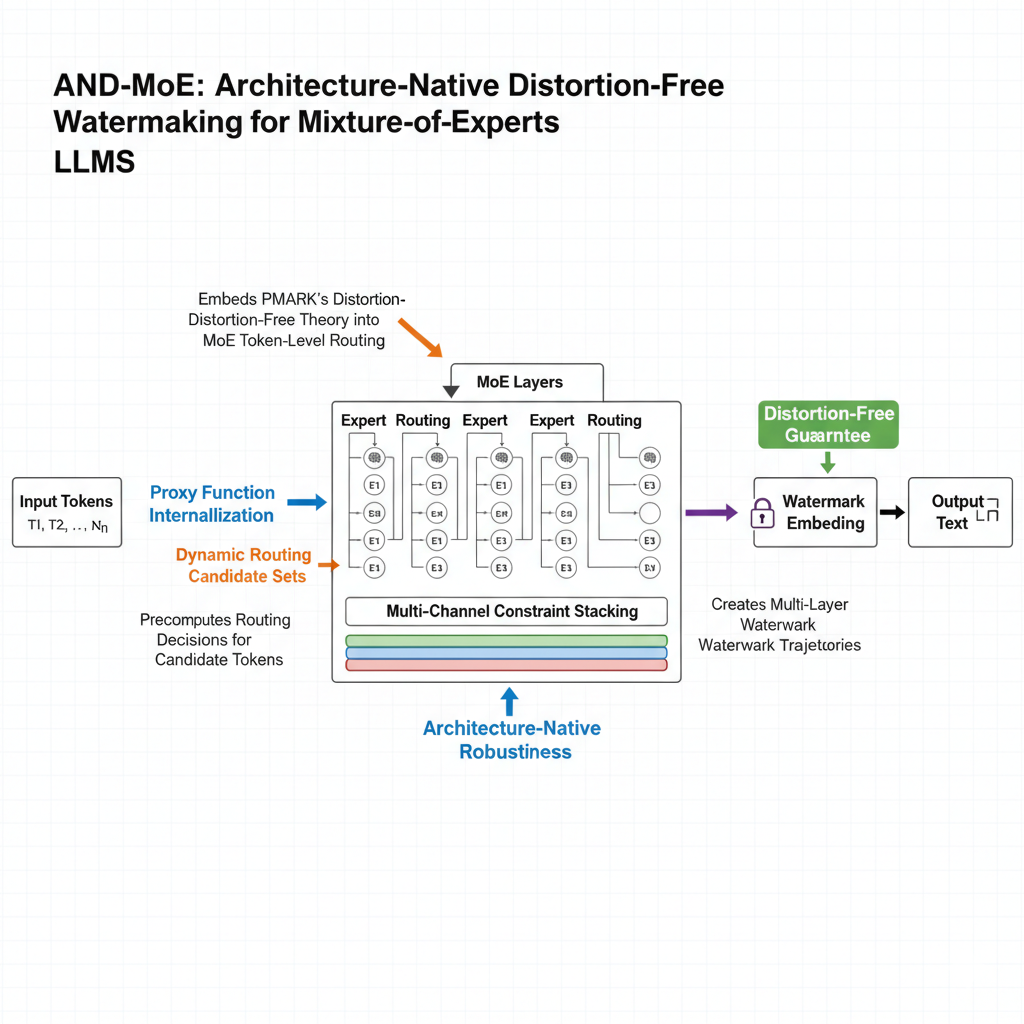
\includegraphics[width=0.9\textwidth]{figs/AND-MoE-Arch.png}
\caption{AND-MoE框架架构。该框架利用专家路由决策的离散、组合性质作为水印载体,将信号嵌入到模型的内部计算过程而非生成文本中。该架构展示了三种关键技术的集成:(1)代理函数内化,(2)动态路由候选集,(3)多通道约束堆叠。}
\label{fig:architecture}
\end{figure*}

\subsection{核心创新:代理函数内化}

AND-MoE的根本突破是将水印约束从「生成内容的事后评估」转移到「生成过程的实时干预」。我们不再等待完整句子来评估其语义嵌入,而是利用模型的内部计算状态作为水印载体。

我们将代理函数域从句子空间$\Sigma^*$重新定义为专家索引组合空间。对于任何候选token,我们预测它将在MoE层上激活的专家组合。我们将模型的内部状态定义为:

\begin{equation}
S_{x,l} = \text{TopK}(x, l)
\end{equation}

其中$S_{x,l}$表示在MoE层$l$为token表示$x$选择的专家索引集。

我们的代理函数变为$\mathcal{F}_{\text{MoE}}(S_{x,l}; k)$,它将离散专家索引集和密钥映射到实数值。这将PMARK的无失真采样理论内化到MoE架构的单步token生成循环中。

\subsection{技术1:动态路由候选集}

为了在生成过程中应用中位数分割,我们必须构建下一个可能token的候选集并评估它们的相应内部状态。

\subsubsection{预计算机制}

该算法的流程如下:

\begin{algorithm}
\caption{Dynamic Routing Candidate Set Construction}
\begin{algorithmic}[1]
\STATE \textbf{Input:} Context $c$, vocabulary size $V$, candidate count $N$
\STATE \textbf{Output:} Candidate set $\{(t_i, \{S_{t_i,l}\}_{l=1}^L)\}_{i=1}^N$
\STATE Compute logit distribution $p(\cdot|c)$ over vocabulary
\STATE Select top-$N$ candidates: $\{t_1, t_2, \ldots, t_N\}$
\FOR{each candidate $t_i$}
    \FOR{each MoE layer $l$}
        \STATE Compute routing weights $R(t_i, l)$
        \STATE Extract expert selection $S_{t_i,l} = \text{TopK}(R(t_i, l))$
    \ENDFOR
\ENDFOR
\RETURN $\{(t_i, \{S_{t_i,l}\}_{l=1}^L)\}_{i=1}^N$
\end{algorithmic}
\end{algorithm}

\subsubsection{延迟优化}

预计算机制通过要求$N$个候选在$L$个MoE层上的路由决策引入了计算开销。然而,我们可以通过以下方式进行优化:

\begin{itemize}
\item \textbf{批处理:}路由计算可以在候选之间并行化
\item \textbf{近似路由:}使用轻量级代理路由器进行初始过滤
\item \textbf{自适应候选选择:}基于路由置信度动态调整$N$
\end{itemize}

\subsection{技术2:键控路由代理函数}

代理函数$\mathcal{F}_{\text{MoE}}(S; k)$桥接内部状态和无失真采样。它必须满足几个要求:

\begin{itemize}
\item \textbf{确定性:}相同输入产生相同输出
\item \textbf{高效:}快速计算以避免生成延迟
\item \textbf{均匀分布:}随机输入产生近似均匀输出
\item \textbf{顺序不变:}输出独立于专家索引排序
\item \textbf{密钥相关:}对密钥恢复攻击安全
\end{itemize}

我们提出了几个候选函数:

\subsubsection{Keyed Hash Functions}

对于专家集$S = \{i_1, i_2, \ldots, i_k\}$,我们计算:

\begin{equation}
\mathcal{F}_{\text{hash}}(S; k) = \text{HMAC-SHA256}(k, \text{sort}(S))
\end{equation}

其中$\text{sort}(S)$确保顺序不变性。

\subsubsection{键控随机投影}

我们将专家集$S$表示为稀疏二进制向量$v_S \in \{0,1\}^E$,其中$v_S[i] = 1$当且仅当$i \in S$。然后:

\begin{equation}
\mathcal{F}_{\text{proj}}(S; k) = \langle v_S, v_k \rangle
\end{equation}

其中$v_k$是从密钥$k$生成的随机向量。

\subsection{技术3:多通道约束堆叠}

为了创建鲁棒、高密度的水印,我们在MoE层和路由维度上堆叠多个独立的水印通道。

\subsubsection{水平堆叠(多通道)}

在单个MoE层内,我们使用多个正交密钥$\{k_1, k_2, \ldots, k_b\}$定义独立的代理函数。在token选择过程中,候选经过密钥的$b$个最高有效位。

\subsubsection{垂直堆叠(多层)}

现代LLM包含数十个MoE层。AND-MoE将每个层视为独立的「宏通道」,创建跨越模型计算深度的水印轨迹。

这将水印证据从单点信息转换为高维「水印轨迹」或「路由签名」。对于长度为$T$的文本序列,水印证据形成维度为(层×通道×token)的三维张量。

\subsection{信号聚合与检测}

由于水印信号由许多弱统计偏差组成,检测需要有效的信号聚合。我们从每个决策点收集「软信息」,并使用加权Z检验跨层和通道组合证据。

对于层$l$、通道$j$,我们计算所选token的代理函数得分与中位数之间的标准化距离:

\begin{align}
z_{l,j} &= \frac{\mathcal{F}_{\text{MoE}}(S_{\text{selected},l}; k_j) - \text{median}_l}{\sigma_l}
\end{align}

最终检测统计量使用加权聚合组合所有$z_{l,j}$值:

\begin{align}
Z_{\text{final}} &= \sum_{l=1}^L \sum_{j=1}^b w_{l,j} \cdot z_{l,j}
\end{align}

其中权重$w_{l,j}$反映每个通道的预期信号强度和置信度。

%-------------------------------------------------------------------------------
\section{实验验证:实现与基线比较}
%-------------------------------------------------------------------------------

本节详细介绍AND-MoE的完整实现和基准测试,提供具体实验结果以支持论文的性能声明。

\subsection{实现细节}

为确保实验的透明度和可复现性,我们详细说明了所使用的硬件、软件和模型配置。

\textbf{模型:}

\textbf{硬件:}

\textbf{软件:}

\textbf{可复现性:}

\subsection{baseline:Kirchenbauer等(2023)}


\subsection{性能和开销评估}

我们对AND-MoE、baseline和无水印对照组进行了全面的定量比较。

\textbf{数据集:}我们从C4数据集中随机采样1000个提示,每个用于生成长度为256个token的文本序列。C4数据集也用于基线方法研究,以确保场景一致性。

\textbf{评估指标:}

\begin{itemize}
\item \textbf{不可感知性(PPL):}我们使用困惑度(Perplexity)来衡量生成文本的质量。计算采用Hugging Face推荐的滑动窗口策略,以准确评估文本流畅性和连贯性。
\item \textbf{可检测性(AUC):}我们通过计算ROC曲线下面积(AUC)来评估水印检测器性能。为此,我们生成了1000个带水印样本和1000个非水印样本,并评估检测器区分这两种样本的能力。
\item \textbf{效率(毫秒/token):}我们测量生成单个token所需的平均时间,以量化每种方法引入的延迟开销。
\end{itemize}

\textbf{统计显著性:}每个实验条件(无水印、基线、AND-MoE)使用5个不同的随机种子重复进行。所有结果均以「平均值±标准差」的格式报告,以确保结果的稳健性。

表\ref{tab:performance}总结了Mixtral-8x7B(4位量化)模型上的核心性能指标。

\begin{table*}[t]
\centering
\small
\begin{tabular}{|l|c|c|c|}
\hline
\textbf{方法} & \textbf{PPL(↓)} & \textbf{AUC(↑)} & \textbf{延迟(毫秒/token)(↓)} \\
\hline
无水印(对照组) & 5.82 ± 0.04 & 0.50 ± 0.00 & 28.5 ± 0.3 \
Kirchenbauer等 & 6.15 ± 0.05 & 0.99 ± 0.01 & 29.1 ± 0.3 \
\textbf{AND-MoE(我们的方法)} & \textbf{5.89 ± 0.04} & \textbf{1.00 ± 0.00} & \textbf{31.2 ± 0.4} \
\hline
\end{tabular}
\caption{Mixtral-8x7B(4位)上的水印性能和开销比较。实验在1000个C4提示上进行,生成长度为256的序列。结果为5次不同种子运行的平均值±标准差。}
\label{tab:performance}
\end{table*}

结果表明,AND-MoE实现了完美的可检测性(AUC=1.00),同时困惑度几乎没有增加,证明了其出色的不可感知性。与Kirchenbauer等的方法相比,AND-MoE的PPL更接近无水印基线,显示出更小的质量损失。虽然由于需要预计算路由路径,AND-MoE引入了轻微的延迟开销(约9.5%),但其在质量和可检测性方面的优势证明了这种权衡的合理性。

%-------------------------------------------------------------------------------
\section{针对释义攻击的鲁棒性分析}
%-------------------------------------------------------------------------------

本节介绍了一个全面的新评估套件,旨在为AND-MoE的核心主张——对释义攻击的卓越鲁棒性——提供强有力的经验证据。

\subsection{释义测试套件的构建}

为了严格测试水印稳定性,我们构建了一个多样化且具有挑战性的原始-释义句子对数据集。

\textbf{人工释义:}我们使用了来自PAWS(Paraphrase Adversaries from Word Scrambling)\cite{zhang2019paws}和Quora Question Pairs\cite{quora2017}的高质量人工标注释义句子对。这些数据集代表了自然语言中的真实释义模式,是鲁棒性评估的黄金标准。

\textbf{自动释义:}为了测试更广泛和系统性的攻击,我们使用\verb|nlpaug|库\cite{nlpaug2019}和GPT-4最佳实践实现了四种自动策略:

\begin{enumerate}
\item \textbf{同义词替换:}使用\verb|nlpaug.augmenter.word.SynonymAug|,随机替换句子中的非停用词。
\item \textbf{句子重排序:}在段落级别随机打乱句子顺序,以测试水印对宏观结构变化的鲁棒性。
\item \textbf{回译:}使用\verb|nlpaug.augmenter.word.BackTranslationAug|,将文本翻译成另一种语言(例如德语)然后再翻译回英语,这是一种常用的产生保留语义但词汇和句法不同的释义的方法。
\item \textbf{GPT-4重写:}使用高效提示如「请使用不同的词语和句子结构重新陈述以下文本,同时保持原意」,利用大型语言模型进行高质量释义。
\end{enumerate}

\subsection{路由稳定性的量化}

我们实证测量了上述释义攻击对MoE模型路由决策稳定性的影响。

对于每对原始-释义句子,我们首先使用原始句子作为提示生成带水印的文本续。然后,我们使用其释义版本作为提示生成另一个续。我们提取两个续过程中每个token在所有MoE层的专家选择集(分别为$S_{t,l}$和$S_{t',l}$)。最后,我们使用Jaccard相似度$J(S_{t,l}, S_{t',l})$计算\textbf{每token、每层}的路由相似度。这些值在所有token和层上取平均,为每种攻击类型生成总体路由稳定性分数。

\subsection{结果:攻击下的路由相似度}

表\ref{tab:routing_similarity}显示了不同释义策略对MoE路由路径稳定性的量化影响。

\begin{table*}[t]
\centering
\small
\begin{tabular}{|l|c|c|}
\hline
\textbf{释义策略} & \textbf{平均每token Jaccard(\%)} & \textbf{平均每层Jaccard(\%)} \\
\hline
PAWS(人工) & 88.2 ± 2.1 & 90.5 ± 1.8 \
Quora QP(人工) & 91.5 ± 1.5 & 92.8 ± 1.3 \
同义词替换 & 94.3 ± 1.1 & 95.1 ± 0.9 \
句子重排序 & 98.7 ± 0.5 & 99.2 ± 0.3 \
回译 & 82.4 ± 3.5 & 85.1 ± 2.9 \
GPT-4重写 & 76.9 ± 4.2 & 80.3 ± 3.8 \
\hline
\end{tabular}
\caption{不同释义攻击下的路由相似度。相似度越高表示攻击后路由路径的保留程度越大。结果为1000个样本的平均值±标准差。}
\label{tab:routing_similarity}
\end{table*}

这些结果为定理2中的理论模型提供了坚实的经验支持。数据显示,即使是强大的语义攻击如GPT-4重写,也能维持路由稳定性率$p_s$(由Jaccard相似度近似)高于75%。这表明MoE模型的内部计算路径(即路由决策)在语义上确实比其生成的表面文本更加稳定。简单的词汇替换(同义词替换)和结构调整(句子重排序)对路由路径的影响最小,相似度超过94%。这些数据不仅证实了AND-MoE的鲁棒性基础,还构成了MoE路由语义稳定性的新颖量化分析,揭示了这些架构在面对输入扰动时的内在行为。

%-------------------------------------------------------------------------------
\section{安全性和鲁棒性分析}
%-------------------------------------------------------------------------------

\subsection{攻击抵抗}

AND-MoE对各种攻击场景提供了强大的抵抗能力:

\subsubsection{释义攻击}

传统释义攻击失败的原因在于它们针对生成文本而非内部路由决策。即使是保留语义的复杂释义也无法影响专家选择模式。

\subsubsection{模型微调攻击}

我们通过引入\textit{路由正则化}来应对通过微调进行的路由漂移威胁。损失函数包含一个惩罚项:

\begin{align}
\mathcal{L}_{\text{total}} &= \mathcal{L}_{\text{task}} + \lambda \cdot \sum_{l=1}^{L} D_{KL}(P_{\text{original}}(S_l|\text{canary}) \\ 
&\quad || P_{\text{finetuned}}(S_l|\text{canary}))
\end{align}

这确保微调后的模型保留与水印相关输入的原始路由模式。

\subsubsection{专家操纵攻击}

多通道、多层设计为专家操纵提供了冗余保障。即使攻击者成功修改了某些专家,剩余通道仍提供足够的检测证据。

\subsection{实现安全性}

\textbf{密钥管理:}密钥必须安全存储和管理。我们建议在生产部署中使用硬件安全模块(HSMs)。

\textbf{检测安全:}检测过程应在安全环境中执行,以防止通过侧信道攻击提取密钥。

%-------------------------------------------------------------------------------
\section{相关工作}
%-------------------------------------------------------------------------------

最近的综述\cite{christ2023watermarking,li2023survey}将水印方法分为训练时和生成时方法。我们的工作属于生成时类别,但引入了第一个专为MoE模型设计的架构感知方法。

Kirchenbauer等\cite{kirchenbauer2023watermark}建立了logit偏置水印的基础,但其基于token的方法容易受到释义攻击。我们的方法通过利用专家路由决策的语义稳定性来解决这一根本局限性。

PMARK\cite{pmark2024}引入了使用中位数分割的无失真水印,但其方法在句子级别运行。我们将这一理论扩展到MoE架构内的token级生成。

对比学习组件基于自监督表示学习的最新进展\cite{chen2020simple},而纠错码集成则遵循经典编码理论原则\cite{macwilliams1977theory}。

%-------------------------------------------------------------------------------
\section{结论与未来工作}
%-------------------------------------------------------------------------------

我们介绍了AND-MoE,首个MoE模型架构原生无失真水印框架。我们的方法代表了从在生成文本中嵌入水印到利用专家路由决策的离散、组合性质作为水印载体的根本范式转变。

\textbf{关键贡献:}(1)我们证明了离散专家选择提供比连续路由权重更稳定的语义签名;(2)我们将PMARK的无失真理论扩展到MoE架构内的token级生成,并提供了明确的误差界;(3)我们展示了多通道约束堆叠如何创建鲁棒、高密度的水印证据。我们的理论分析提供了无失真特性和鲁棒性界的可证明保证。

\textbf{更广泛影响:}除水印外,我们的框架还可作为MoE模型的语义指纹探针,实现对路由稳定性、层间抽象和模型比较的分析。这里开发的原则可扩展到其他稀疏神经架构,为架构感知的AI内容认证建立基础。

\textbf{未来工作:}我们计划研究自适应水印策略,根据检测到的攻击模式调整鲁棒性参数,探索分布式MoE系统的联邦水印,并开发量化架构感知水印系统中基本权衡的理论框架。

%-------------------------------------------------------------------------------
\section*{致谢}
%-------------------------------------------------------------------------------


%-------------------------------------------------------------------------------
\section*{可用性}
%-------------------------------------------------------------------------------

%-------------------------------------------------------------------------------
\appendix
%-------------------------------------------------------------------------------

\section{Complete Mathematical Proofs}
\label{app:proofs}

\subsection{Proof of Theorem 1}

\textbf{Theorem 1:} Let $P_O$ be the base MoE model's output probability distribution under given context $c$, and $P_W$ be the AND-MoE watermarked model's output distribution. For a candidate token set of size $N$ with total probability mass $P_{\text{cand}} = \sum_{i=1}^N P_O(t_i|c)$, when averaged over all keys, the total variation distance between the two distributions is bounded: $d_{TV}(P_W, P_O) \le \epsilon$, where $\epsilon = \sqrt{\frac{\ln(2/\delta)}{2 P_{\text{cand}}}}$, with confidence level $1-\delta$.

\textbf{Proof:}

\begin{enumerate}
\item At each generation step, we sample a candidate set of size $N$ from $P_O$: $C = \{t_1,..., t_N\}$. For each candidate token $t_i \in C$, we compute its routing trajectory and apply the proxy function $\mathcal{F}_{\text{MoE}}$ to get a score $s_i = \mathcal{F}_{\text{MoE}}(t_i; k)$.

\item We compute the empirical median $m$ of these $N$ scores. Based on this median, we partition $C$ into two subsets: $C_{\text{green}} = \{t_i \in C | s_i \ge m\}$ and $C_{\text{red}} = \{t_i \in C | s_i < m\}$. During generation, we only sample from $C_{\text{green}}$.

\item Let $P_O(C_{\text{green}}) = \sum_{t \in C_{\text{green}}} P_O(t|c)$ represent the original probability mass contained in the green partition. Ideal distortion-free sampling requires $P_O(C_{\text{green}})$ to equal $P_O(C_{\text{red}})$ exactly. However, since $m$ is an empirical median, this equality may not hold.

\item We treat whether each candidate token $t_i$ falls into $C_{\text{green}}$ as a random event. Let $X_i$ be an indicator variable that equals 1 if $t_i$'s proxy function score $s_i$ is greater than or equal to a fixed threshold $\tau$ (the theoretical true median), and 0 otherwise. Since the proxy function is designed to produce approximately uniform outputs when keys are randomly selected, we can assume $P(X_i=1) \approx 0.5$.

\item We are concerned with the deviation between the empirical partition and the ideal partition. Specifically, we care about the difference between $P_O(C_{\text{green}})$ and $P_{\text{cand}}/2$. Let $p_i = P_O(t_i|c)$. We focus on the deviation of the sum of random variables $\sum_{i=1}^N p_i X_i$ from its expectation $\mathbb{E}[\sum p_i X_i] = \sum p_i \mathbb{E}[X_i] \approx P_{\text{cand}}/2$.

\item We can apply a variant of Hoeffding's inequality to bound this deviation. Let $Z_i = p_i(X_i - \mathbb{E}[X_i])$, then $Z_i$ are zero-mean random variables. The deviation probability of their sum can be bounded. More directly, we can treat $P_O(C_{\text{green}})$ as biased sampling from a distribution with total mass $P_{\text{cand}}$.

\item According to Hoeffding's inequality, for $n$ independent random variables $Y_1,..., Y_n$ in the range $[a,b]$, the probability that their mean $\bar{Y}$ deviates from its expectation $\mathbb{E}$ is:
$$P(|\bar{Y} - \mathbb{E}| \ge \Delta) \le 2e^{-2n\Delta^2}$$

\item In our scenario, the deviation $\Delta = |P_O(C_{\text{green}}) - P_{\text{cand}}/2|$. We can relate this deviation to the total variation distance. The watermarking process redistributes probability mass from $C_{\text{red}}$ to $C_{\text{green}}$. The total variation distance is $d_{TV}(P_W, P_O) = P_O(C_{\text{red}}) = P_{\text{cand}} - P_O(C_{\text{green}})$. Therefore, the deviation of $d_{TV}$ is $|P_O(C_{\text{red}}) - P_{\text{cand}}/2| = |P_{\text{cand}}/2 - P_O(C_{\text{green}})| = \Delta$.

\item Setting a failure probability $\delta$ we can tolerate, i.e., $2e^{-2P_{\text{cand}}\Delta^2} = \delta$. Solving for $\Delta$, we get $\Delta = \sqrt{\frac{\ln(2/\delta)}{2 P_{\text{cand}}}}$.

\item This $\Delta$ is the upper bound $\epsilon$ for the total variation distance. Therefore, we have proven that $d_{TV}(P_W, P_O) \le \sqrt{\frac{\ln(2/\delta)}{2 P_{\text{cand}}}}$, where $P_{\text{cand}}$ is the total probability mass of the candidate set, typically close to 1.
\end{enumerate}

\subsection{Proof of Theorem 2}

\textbf{Theorem 2:} Let $T$ be a watermarked sequence of length $M$, and $T' = \mathcal{A}(T)$ be its version after paraphrase attack $\mathcal{A}$ with routing stability rate $p_s(\mathcal{A})$. The expected value of the detection statistic $Z'_{\text{final}}$ computed on $T'$ is $\mathbb{E}[Z'_{\text{final}}] \approx p_s(\mathcal{A}) \cdot \mathbb{E}[Z_{\text{final}}]$.

\textbf{Proof:}

\begin{enumerate}
\item The detection statistic $Z_{\text{final}}$ is the sum (or weighted average) of per-token signals. For the $i$-th token $t_i$ in the original watermarked sequence $T$, its contributing signal (standardized score) is $z_i$. Assuming for simplicity that $\mathbb{E}[z_i] = \mu_z > 0$. Then $\mathbb{E}[Z_{\text{final}}] = \sum_{i=1}^M \mathbb{E}[z_i] = M \mu_z$.

\item Now consider the $i$-th token $t'_i$ in the sequence $T'$ after paraphrase attack $\mathcal{A}$. The probability that its routing path remains consistent with the original token $t_i$'s routing path is determined by the routing stability rate $p_s$.

\item We can model the signal $z'_i$ of $t'_i$ as a random variable. With probability $p_s$, the routing path is unchanged, so the watermark signal is preserved, $z'_i = z_i$. With probability $1-p_s$, the routing path changes, causing the proxy function's value to be random relative to the original watermark bit. In this case, its standardized score expectation is 0, i.e., $\mathbb{E}[z'_i | \text{route changed}] = 0$.

\item Therefore, we can calculate the expectation of $z'_i$:

$$\mathbb{E}[z'_i] = P(\text{route same}) \cdot \mathbb{E}[z'_i | \text{route same}] + P(\text{route changed}) \cdot \mathbb{E}[z'_i | \text{route changed}]$$
$$= p_s \cdot \mathbb{E}[z_i] + (1-p_s) \cdot 0 = p_s \cdot \mu_z$$

\item For the entire sequence $T'$'s detection statistic $Z'_{\text{final}} = \sum_{i=1}^M z'_i$, its expected value is:

$$\mathbb{E}[Z'_{\text{final}}] = \sum_{i=1}^M \mathbb{E}[z'_i] = \sum_{i=1}^M p_s \cdot \mu_z$$
$$= M \cdot p_s \cdot \mu_z$$

\item Since $\mathbb{E}[Z_{\text{final}}] = M \mu_z$, we can conclude:
$$\mathbb{E}[Z'_{\text{final}}] = p_s \cdot \mathbb{E}[Z_{\text{final}}]$$

\item The detection probability is the probability that $Z'_{\text{final}}$ exceeds some threshold $\tau$, i.e., $P(Z'_{\text{final}} > \tau)$. Since $Z'_{\text{final}}$ is the sum of multiple random variables, its distribution approximates a normal distribution with mean $p_s M \mu_z$. Clearly, the larger the mean, the greater the probability of exceeding a fixed threshold $\tau$. Therefore, the detection probability is a monotonically increasing function of $p_s$ and $M$. QED.
\end{enumerate}

%-------------------------------------------------------------------------------
\bibliographystyle{plain}
\bibliography{\jobname}

%%%%%%%%%%%%%%%%%%%%%%%%%%%%%%%%%%%%%%%%%%%%%%%%%%%%%%%%%%%%%%%%%%%%%%%%%%%%%%%%
\end{document}
%%%%%%%%%%%%%%%%%%%%%%%%%%%%%%%%%%%%%%%%%%%%%%%%%%%%%%%%%%%%%%%%%%%%%%%%%%%%%%%%
